\documentclass[UTF8]{ctexart}


% \lstset{frame=, basicstyle={\footnotesize\ttfamily}}



% \graphicspath{ {images/} }
\usepackage{ctex}
\usepackage{minted}
\usepackage{graphicx}
\usepackage{pdflscape}
\usepackage{titlesec}
\usepackage{float}
\usepackage[export]{adjustbox}
\usepackage[colorlinks, 
            linkcolor=black,
            anchorcolor=black,
            citecolor=black]{hyperref}

\setcounter{secnumdepth}{4}

\titleformat{\paragraph}
{\normalfont\normalsize\bfseries}{\theparagraph}{1em}{}
\titlespacing*{\paragraph}
{0pt}{3.25ex plus 1ex minus .2ex}{1.5ex plus .2ex}
%-----------------------------------------BEGIN DOC----------------------------------------

\begin{document}
\renewcommand{\contentsname}{目\ 录}
\renewcommand{\appendixname}{附录}
% \renewcommand{\appendixpagename}{附录}
\renewcommand{\refname}{参考文献} 
\renewcommand{\figurename}{图}
\renewcommand{\tablename}{表}
\renewcommand{\today}{\number\year 年 \number\month 月 \number\day 日}

\title{{\Huge U10M11007试点班实验报告{\large\linebreak\\}}{\Large 三级流水线设计报告\linebreak\linebreak}}
%please write your name, Student #, and Class # in Authors, student ID, and class # respectively
\author{\\姓\ 名:王\ 嘉\ 利\\
学\ 号: 2018302278\\
班\ 号: 10011801\\\\
CS 11007 计算机组成与体系结构\\
(春季, 2020)\\\\
西北工业大学\\
计算机学院\\
ERCESI}
\date{\today}
\maketitle
\newpage

%-----------------------------------------ABSTRACT-------------------------------------
\begin{center}
{\Large\bf{摘\ 要\\}}
\end{center}
本次实验在分析SMIPA指令集的基础上设计了三级流水处理器。将指令的执行分为取指、译码、执行访存写回三个阶段。
设计了三级流水的数据通路和控制通路,分析了数据冒险、控制冒险和例外执行时的特征。最后列出了模块所需的接口。
\newpage
%-----------------------------------------ABSTRACT-------------------------------------
\begin{center}
{\Large\bf{版\ 权\ 声\ 明\\}}
\end{center}
该文件受《中华人名共和国著作权法》的保护。ERCESI实验室保留拒绝授权违法复制该文件的权利。任何收存和保管本文件各种版本的单位和个人,未经ERCESI实验室(西北工业大学)同意,不得将本文档转借他人,亦不得随意复制、抄录、拍照或以任何方式传播。 否则,引起有碍著作权之问题,将可能承担法律责任。\newpage
%-----------------------------------------CONTENT-------------------------------------
\begin{center}
\tableofcontents\label{c}
\end{center}
\newpage

%------------------------------------------TEXT--------------------------------------------

%----------------------------------------OVERVIEW-----------------------------------------

\section{概述} \label{overview}%------------------------------
三级流水处理器将指令的执行分为三个阶段。在第一个阶段,PC从指令内存中取出指令;
第二阶段,将指令进行译码;第三阶段完成剩余的步骤。在出现冒险或者异常的情况下,流水线正常流,一拍一个指令。
在处理跳转指令时,预测下一个指令就是PC+4,并且将跳转目标的计算放在译码级,
当出现控制冒险的时候,清空流水线从新的地址取值;由于三级流水的特点,简化了数据冒险;对于例外来讲,MIPS是
精确异常,异常指令前面的指令都处理结束,异常的提交是在流水线的最后一级,而且例外也可以看成一个控制冒险,流水线的
清空都通过控制冒险单元完成。


%----------------------------------SYSTEM DESIGN------------------------------------------

\begin{landscape}
    
    \begin{figure}[]
        \centering
        % \flushleft    
        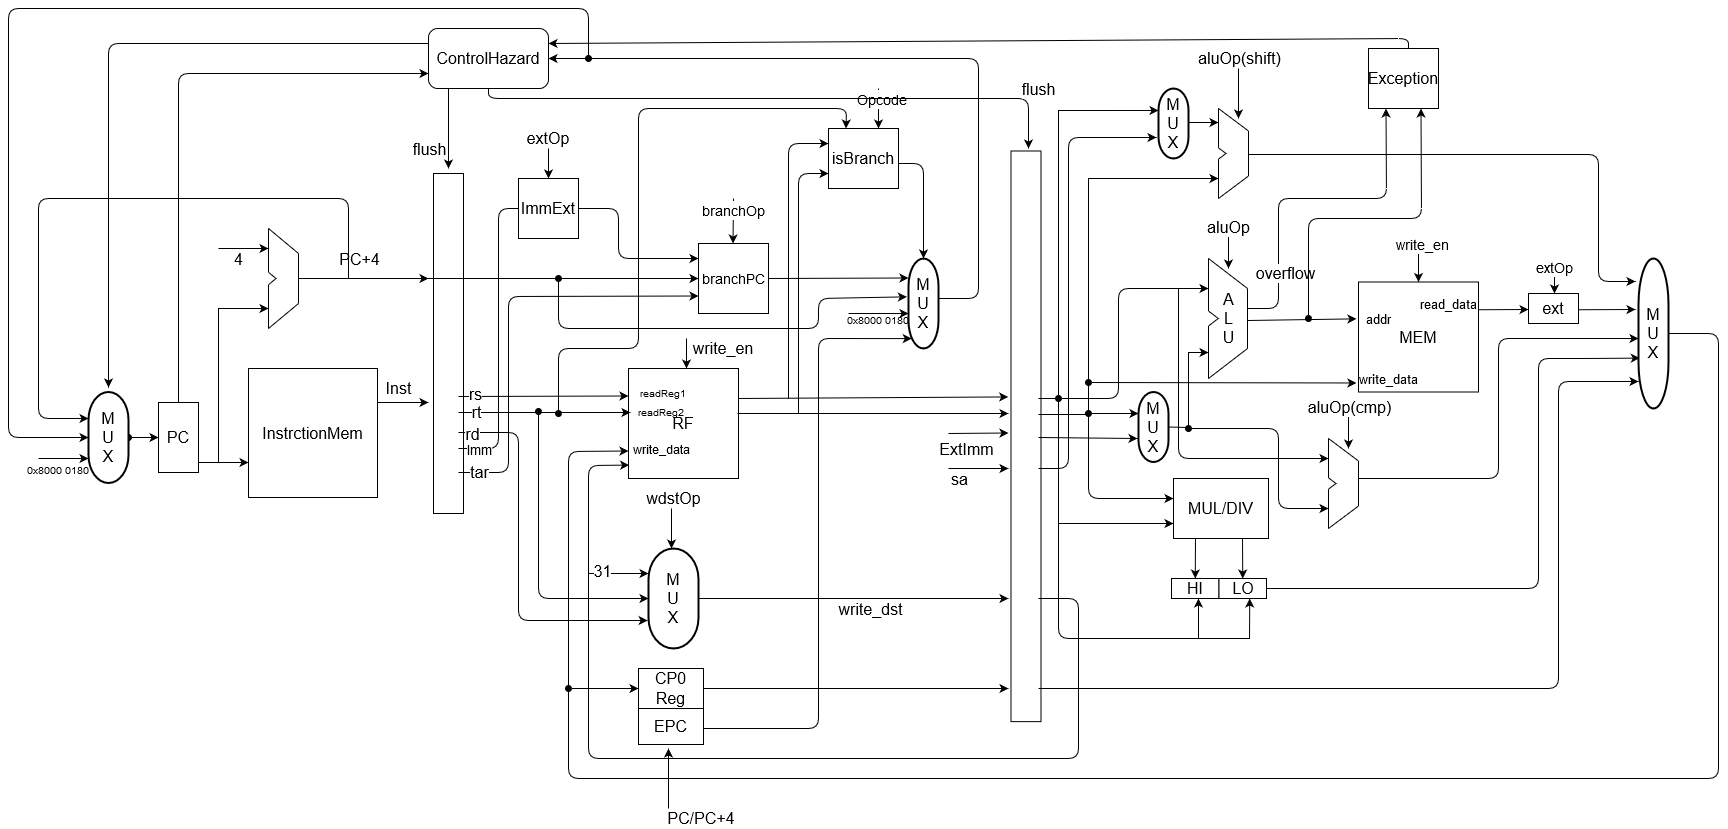
\includegraphics[ width=270mm,center]{3-stages-pipeline.png}
        \caption{三级流水处理器结构图}
        \label{fig:singleblock}
    \end{figure}
    \end{landscape}
\newpage
\section{系统设计} \label{sysdes}%------------------------------
\subsection{System Overview}\label{sub:sysover}
三级流水线处理器的结构图如上图所示
\subsection{数据通路}
\begin{itemize}
    \item{\textbf{取指}\   PC从InstructionMemory从取出指令交给下一个阶段译码。
    而PC可能的取值是PC+4、跳转的地址、异常处理的地址,也有可能来自EPC,因此要用多选器选出PC的值,
    再从InstructionMemory中取出指令。但是在取值的时候并不知道nextPC是多少,因此,
    就采用静态分支预测,预测nextPC每次都是PC+4}
    \item{\textbf{译码}\  在这一阶段,需要将执行指令时可能用到的数据准备好,对立即数进行扩展等。另外,因为第三阶段的数据通路比较长,所以可以将判断是否跳转放到译码阶段,尽可能更早知道是否要跳转}
    \item{\textbf{执行访存和写回}\ \  在执行指令时,可以把运算分为移位、算术逻辑运算、比较运算,以及乘除法;在访存时,
    访存的地址一定是来自算术运算的结果,写入的数据是rt的值;对于
    写回,写回寄存器的数据是来自执行和访存的输出,或者是HiLo寄存器。在译码时产生一信号,对写入的数据进行选择}
    % \item{\textbf{使用Chisel3描述结构} Chisel是一种强大的结构化硬件描述语言,可以对模块、接口以及操作等进行高效率的描述,与Verilog语言相比较,对电路的结构属性具有更好的封装,对系统的描述更加简化。我们选择Chisel3是因为在Linux系统中,使用Chisel3完全不再依赖工业EDA软件实现电路的逻辑仿真,更有利于学术研究和教学应用。虽然Chisel语法在不同版本差异不大,但是部分修饰符的描述方式仍然具有差别,详细区别请参考: \url{https://github.com/ucb-bar/chisel3/wiki/Chisel3-vs-Chisel2}.}
\end{itemize}
\subsection{控制通路}
控制主要是通过\mintinline{c}{opcode} \ \mintinline{c}{func}解码出来的信号来进行控制的。
每拍将相应的控制信号送到后面的流水线寄存器。
对ALU来讲,控制比较有特点,因为将ALU分成了三个功能不同的ALU,所以
总体上可以直接将\mintinline{c}{opcode}段 \ \mintinline{c}{func}段的后三位来进行控制
关于EPC写入数据的选择信号来自trap信号(异常是否是自陷),如果是选择PC+4,否则PC。
\subsection{冒险}
\subsubsection{数据冒险}
考虑最简单的情况\ref{chart:dHazard},第二条指令h和第一个指令相关,
and指令在译码阶段要用到add的执行结果,此时RF的写使能和和读是同时存在的,
可以认为RF内部进行了forward,消除了冒险。同理,可以发现,对一个寄存器的累加操作,
即连续的\mintinline{s}{add $1,$1,$2}类似这样的操作,也不会出现冒险。再来考虑,需要的数据是lowd
指令从MEM中取出来的,因为执行和访存是同一个阶段,因此也没有冒险。
\begin{table}[h]
    \centering
    \begin{tabular}{|c|c|c|c|c|c|}
        \hline
        & C1 & C2 & C3 & C4 & C5  \\ \hline 
    \mintinline{s}{add $1,$2,$3} & F & D & EMW & &  \\ \hline 
    \mintinline{s}{and $2,$1,$4} &   & F & D & EMW & \\ \hline 
    \mintinline{s}{or  $5,$1,$3}  &  &    & F & D & EMW  \\ \hline 
    \end{tabular}
    \caption{data hazard}\label{chart:dHazard}
\end{table}


     可以发现在一般情况下,对于这种三级流水线都不会产生数据冒险
\subsubsection{控制冒险和异常} 控制冒险可以分成两类,一个是由于例外造成的,一个是由于分支预测错误造成的。

先来考虑由于分支预测错误造成的冒险,首先把是否冒险探测出来,因为将nextPC的计算提前,放到了译码阶段,因此通过
检测取指的PC和译码时产生的nextPC是否相等就可以判断出是否有冒险产生。如果预测失败,
那么就清空给取指的指令,PC的值选择为nextPC。这个通过一个单独的控制冒险单元实现。

再来考虑异常。首先考虑异常的产生情况,一种是自陷指令(\mintinline{s}{break syscall}),指令的目的就是为了产生
异常,另一种是ALU算出来的结果溢出,或者是算出来的地址不正确。对于第一个,在译码阶段就可以发现,把这个异常信号
记在流水线里,在最后一级流水线时提交。第二种异常,在第三级流水时产生,而且不希望错误的结果写回到寄存器或者
存储器。用一个异常单元对异常进行检测和处理,处理异常时需要清空流水线,将异常原因写到cause寄存器,而且要根据不同的异常
将EPC的值设为PC或者PC+4。清空流水线和和跳转到异常处理地址,可以通过控制冒险单元完成。

\textbf{e.g. 1} 
\begin{minted}{s}
    add $1,$2,$3
    beq $1,$2,100
    lw $3, 0($4)
    ...
    or $2,$1,$3 // 跳转目标
\end{minted}
\begin{table}[h]
    \begin{minipage}{1\linewidth}
        \centering
        \begin{tabular}{|c|c|c|c|}
            \hline
            & C1 & C2 & C3   \\ \hline 
        \mintinline{s}{add $1,$2,$3} & F & D & EMW   \\ \hline 
        \mintinline{s}{beq $1,$2,100} &   & F & D  \\ \hline 
        \mintinline{s}{lw $3, 0($4)}  &  &    & F   \\ \hline 
        \end{tabular}
        \centerline{(a)探测到冒险}
    \end{minipage}
    \vfill
    \begin{minipage}{1\linewidth}
        \centering
        \begin{tabular}{|c|c|c|c|c|c|}
            \hline
            & C1 & C2 & C3 & C4 & C5  \\ \hline 
        \mintinline{s}{add $1,$2,$3} & F & D & EMW & &   \\ \hline 
        \mintinline{s}{beq $1,$2,100} &  & F & D & EMW &  \\ \hline 
        \mintinline{s}{lw $3, 0($4)}  &  &   & F & buble & buble  \\ \hline 
        \mintinline{s}{or $2,$1,$3}   &  &   &   & F  & D \\ \hline
        \end{tabular}
        \centerline{(b)处理冒险}
    \end{minipage}
\end{table}

\textbf{e.g. 2}
\begin{minted}{s}
    break 
    beq $1,$2, 100 // branch take
    and $1,$2,$3
\end{minted}
要考虑这种情况,当break进入最后一级流水时,发现了异常,ID级流水同时也发现了分支预测错误。但是
应该ControlHazard单元因该处理异常而不是分支预测错误。
\begin{minted}{python}
    if exception and nextPC != PC :
        PCSrc should choose ExceptionHandling address
\end{minted}
% -----------------------------------BLOCKS DESIGN----------------------------------------
\section{模块详细设计}
\subsection{数据通路相关}
\subsubsection{ImmExt 扩展单元} 
\paragraph{功能描述} 
对16bits立即数进行扩展
\paragraph{接口定义}
\begin{table}[h]
    \centering
    \begin{tabular}{|c|c|c|c|}
        \hline  
        名称 & 位宽 & 方向 & 描述 \\ \hline 
        imm  & 16 & in & 立即数\\ \hline 
        extImm & 32 & out & 扩展后的立即数 \\ \hline
        extOp & 1 & in & 符号还是无符号扩展\\ \hline
    \end{tabular}
    \caption{ImmExt 接口}
\end{table}

\paragraph{逻辑控制}
可以发现,只有逻辑运算时才进行无符号扩展,进一步可以用\mintinline{c}{opcode[3]&opcode[2]}作为extOp
\begin{table}[h]
    \centering
    \begin{tabular}{|c|c|c|}
        \hline
        extOp & 0 & 1 \\ \hline
        扩展  & signed & unsigned \\ \hline
    \end{tabular}
\end{table} \\
\subsubsection{branchPC }
用来计算跳转的地址。
\begin{table}[h]
    \centering
    \begin{tabular}{|c|c|c|c|}
        \hline  
        名称 & 位宽 & 方向 & 描述 \\ \hline 
        extImm & 32 & in & 扩展后的立即数 \\ \hline
        PC & 32 & in & pc \\ \hline 
        target & 32 & in & J,JR等指令的跳转目标 \\ \hline 
        branchOp & 1 & in & 控制信号 \\ \hline
        branchPC & 32 & out & 跳转目标\\ \hline
    \end{tabular}
\end{table}
branchOp控制跳转地址的计算,通过\mintinline{c}{opcode[2:0]}产生这个信号。如果
\mintinline{c}{opcode[2:0]}是0,2,3输出是target,否则是extImm与PC相加的结果。
\subsubsection{isBranch}
用来产生next PC的选择信号
\begin{table}[h]
    \centering
    \begin{tabular}{|c|c|c|c|}
        \hline  
        名称 & 位宽 & 方向 & 描述 \\ \hline 
        valA & 32 & in & R[rs] \\ \hline
        valB & 32 & in & R[rt] \\ \hline 
        rt & 5 & in & branch指令的rt段 \\ \hline 
        opcode & 6 & in & 控制信号 \\ \hline
        PCSel & 2 & out & nextPC的选择信号\\ \hline
    \end{tabular}
\end{table}
\subsubsection{Reg File}
\paragraph{功能描述}
32个通用寄存器堆,实现寄存器的读写
\paragraph{接口定义}
\begin{table}[h]
    \centering
    \begin{tabular}{|c|c|c|c|}
        \hline  
        名称 & 位宽 & 方向 & 描述 \\
        \hline  
        readReg1 & 5 & in &  读寄存器1 \\ \hline
        readReg2 & 5 & in & 读寄存器2 \\ \hline
        write\_data & 32 & in & 写数据 \\ \hline
        writeReg & 5 & in & 写寄存器 \\ \hline
        write\_en & 1 & in & 写使能 \\ \hline
        read\_data1 & 32 & out & 读数据 \\ \hline 
        read\_data2 & 32 & out & 读数据 \\ \hline

    \end{tabular}
    \caption{RF接口}
\end{table}
\paragraph{逻辑控制}
因为受到冒险和异常的影响,需要能够清空流水线,所以write\_en的控制会较其他信号复杂一些
当发现有控制冒险,或者在在执行指令时发现异常,应该让相应指令的write\_en置零
\subsubsection{ALU}\label{sub:alu}
\paragraph{功能描述}
\begin{itemize}
    \item \textbf{算术、逻辑运算ALU}\  用来进行算术运算与逻辑运算,处理类似\mintinline{c}{ADD AND}这类指令
    \item \textbf{移位运算ALU}\  用来进行移位运算, 处理类似于\mintinline{c}{SLL SRL} 这类指令 
    \item \textbf{比较运算ALU} \ 用来进行比较, 处理类似于\mintinline{c}{SLT}这类指令
\end{itemize}
\paragraph{接口定义}
\textbf{算术、逻辑运算ALU}
\begin{table}[h]
    \centering
    \begin{tabular}{|c|c|c|c|}
        \hline  
        名称 & 位宽 & 方向 & 描述 \\
        \hline  
        alu\_A & 32 & in & ALU的操作数 \\
        \hline 
        alu\_B & 32 & in & ALU的操作数 \\
        \hline 
        aluOp & 3 & in & ALU控制信号 \\
        \hline
        alu\_out & 32 & out & ALU计算输出 \\
        \hline
        overflow & 1 & out & 整数溢出标志 \\
        \hline
    \end{tabular}
    \caption{ALU接口}
\end{table}

\textbf{移位运算ALU 比较运算ALU}
剩下两个ALU模块的接口是一样的
\begin{table}[h]
    \centering
    \begin{tabular}{|c|c|c|c|}
        \hline  
        名称 & 位宽 & 方向 & 描述 \\
        \hline  
        alu\_A & 32 & in & ALU的操作数 \\
        \hline 
        alu\_B & 32 & in & ALU的操作数 \\
        \hline 
        aluOp & 3 & in & ALU控制信号 \\
        \hline
        alu\_out & 32 & out & ALU计算输出 \\
        \hline

    \end{tabular}
    \caption{ALU接口}
\end{table}

\paragraph{逻辑控制} 
\textbf{算术、逻辑运算ALU} \\
\begin{table}[h]
    \centering
    \begin{tabular}{|c|c|c|c|c|c|c|c|c|}
        \hline
        aluOp & 000 & 001 & 010 & 011 & 100 & 101 & 110 & 111 \\ \hline
        运算  & ADD & ADDU & SUB & SUBU & AND & OR & NOR & XOR \\ \hline
    \end{tabular}
    \caption{ALU控制}
\end{table} \\
ALU的两个操作数一个是来自rs,一个来自rt或者立即数。用\mintinline{c}{opcode[5:3]}来选择
\begin{minted}{c}
    if opcode[5:3] == 000 :
        alu_B = R[rt]
    else :
        alu_B = extImm 
\end{minted}

\textbf{移位运算ALU} \\
\begin{table}[h]
    \centering
    \begin{tabular}{|c|c|c|c|c|c|c|c|c|}
        \hline
        aluOp & 000 & 001 & 010 & 011 & 100 & 101 & 110 & 111 \\ \hline
        运算  & SLL & xxx & SRL & SRA & SLLV & xxx & SRLV & SRAV \\ \hline
    \end{tabular}
        \caption{ALU控制(xxx是不关心的情况)}
\end{table}\\
这些移位指令都是R-type指令,ALU的操作数alu\_B来自rt,alu\_A来自R[rs]或者sa
\begin{minted}{c}
    alu_A = func[3] ? R[rt] : sa
\end{minted}

\textbf{比较运算ALU} \\
\begin{table}[h]
    \centering
    \begin{tabular}{|c|c|c|c|}
        \hline
        aluOp & 010 & 011 & other\\ \hline
        运算  & signed cmp & unsigned cmp  & xxx \\ \hline
    \end{tabular}
        \caption{ALU控制(xxx是不关心的情况)}
\end{table}\\
ALU的操作数和算术逻辑ALU的操作数一致

\subsubsection{InstMEM  MEM}
\paragraph{指令内存}
\begin{table}[h]
    \centering
    \begin{tabular}{|c|c|c|c|}
        \hline  
        名称 & 位宽 & 方向 & 描述 \\ \hline
        inst\_sram\_en & 1 & in & 使能信号 \\ \hline 
        inst\_sram\_wen& 4 & in & 写使能 \\ \hline 
        inst\_sram\_addr & 32 & in & 读写地址 \\ \hline 
        inst\_sram\_wdata & 32 & in & 写数据 \\ \hline 
        inst\_sram\_rdata & 32 & out & 写数据 \\ \hline
    \end{tabular}
\end{table}
\paragraph{数据内存}
\begin{table}[h]
    \centering
    \begin{tabular}{|c|c|c|c|}
        \hline  
        名称 & 位宽 & 方向 & 描述 \\ \hline
        data\_sram\_en & 1 & in & 使能信号 \\ \hline 
        data\_sram\_wen& 4 & in & 写使能 \\ \hline 
        data\_sram\_addr & 32 & in & 读写地址 \\ \hline 
        data\_sram\_wdata & 32 & in & 写数据 \\ \hline 
        data\_sram\_rdata & 32 & out & 写数据 \\ \hline
    \end{tabular}
\end{table}
\subsection{控制通路相关}
\subsubsection{ControlHazard}
探测和处理控制冒险
\begin{table}[h]
    \centering
    \begin{tabular}{|c|c|c|c|}
        \hline  
        名称 & 位宽 & 方向 & 描述 \\ \hline
        PC & 32 & in & PC寄存器中的值 \\ \hline
        nextPC & 32 & in & 计算出的nextPC \\ \hline
        exception & 1 & in & 异常标志 \\ \hline 
        PCSrc & 2 & out & PC的选择信号 \\ \hline 
        IF\_flush & 1 & out & 清空IF信号 \\ \hline 
        ID\_flush & 1 & out & 清空ID信号 \\ \hline
    \end{tabular}
\end{table}\\
清空ID流水可以将写信号置零,对于IF则插入一个nop指令
\subsubsection{Exception}
对异常进行探测和处理
\begin{table}[h]
    \centering
    \begin{tabular}{|c|c|c|c|}
        \hline  
        名称 & 位宽 & 方向 & 描述 \\ \hline
        trap & 1 & in & 自陷指令异常标志 \\ \hline
        overflow & 1 & in & 整数溢出异常标志 \\ \hline 
        addrFault & 1 & in & 地址错异常标志 \\ \hline     
        cause & 32 & out & 写到Cause寄存器的原因 \\ \hline 
        exception & 1 & out & 异常标志 \\ \hline
    \end{tabular}
    
\end{table}\\
addrFault信号来自判读是否地址错单元的输出。
%add more subsections for other block in you CPU design.
\subsection{流水级顶层module}
\subsubsection{IF}
\begin{table}[h]
    \centering
    \begin{tabular}{|c|c|c|c|}
        \hline  
        名称 & 位宽 & 方向 & 描述 \\ \hline
        nextPC & 32 & in & 计算出的nextPC \\ \hline
        PCSRc & 2 & in & PC选择信号 \\ \hline
        flush & 1 & in & 清空信号 \\ \hline 
        IM\_en & 1 & in & instMem 使能 \\ \hline
        PC & 32 & out & PC值  \\ \hline
        PC4 & 32 & out & PC+4 \\ \hline 
        Inst & 32 & out & 指令 \\ \hline 
    \end{tabular}
    \caption{IF接口}
\end{table}
\subsubsection{ID}
因为考虑后面的流水级可能要使用关于Inst的信息,所以直接将Inst传到流水线寄存器。而且对于
一些信号是要从第三级流水拉回来,同名的信号也会在译码产生,用in和out后缀来区分。
\begin{table}[h]
    \centering
    \begin{tabular}{|c|c|c|c|}
        \hline  
        名称 & 位宽 & 方向 & 描述 \\ \hline
        Inst & 32 & in & 指令 \\ \hline
        PC4\_in(out) & 32 & in(out) & PC+4 \\ \hline
        PC\_in(out) & 32 & in(out) & PC  \\ \hline
        write\_dst\_in(out) & 5 & in(out) & 寄存器目标 \\ \hline
        write\_reg\_in(out) & 1 & in(out) & RF写使能 \\ \hline
        write\_reg\_data & 32 & in & 写会寄存器的值 \\ \hline 
        write\_epc & 1 &in & 写EPC使能 \\ \hline 
        write\_cp0reg\_in(out) & 1 & in(out) & 写CP0寄存器使能  \\ \hline
        flush & 1 & in & 清空信号 \\ \hline 
        reg\_data1 & 32 & out & 寄存器读数据 \\ \hline 
        reg\_data2 & 32 & out & 寄存器读数据 \\ \hline
        extImm & 32 & out & 扩展后的立即数 \\ \hline
        % write_dst_out & 5 & out & 译码得到的写寄存器目标 \\ \hline
        nextPC & 32 & out & 下一个PC \\ \hline
        Inst & 32 & out & 指令 \\ \hline
        write\_hilo & 1 & out & HI LO写使能 \\ \hline
        write\_mem & 4 & out & 写DMem使能 \\ \hline
        trap & 1 & out & 是否出现自陷指令 \\ \hline 
        extOp & 2 & out & MEM读出数据后的扩展控制信号 \\ \hline
        write\_data\_src & 3 & out & 写会数据的选择信号 \\ \hline
    \end{tabular}
    \caption{ID接口}
\end{table}\\
必要的控制信号也要输出
\subsubsection{EMW}
EMW的输入基本都来自于ID级译码的结果
\begin{table}[h]
    \centering
    \begin{tabular}{|c|c|c|c|}
        \hline  
        名称 & 位宽 & 方向 & 描述 \\ \hline
        Inst & 32 & in & 指令 \\ \hline
        PC4\_in(out) & 32 & in(out) & PC+4 \\ \hline
        PC\_in(out) & 32 & in(out) & PC  \\ \hline
        reg\_data1 & 32 & in & 寄存器读数据 \\ \hline 
        reg\_data2 & 32 & in & 寄存器读数据 \\ \hline
        write\_hilo & 1 & in & HI LO写使能 \\ \hline
        write\_mem & 4 & in & 写DMem使能 \\ \hline
        DM\_en & 1 & in & DMem使能 \\ \hline
        trap & 1 & in & 是否出现自陷指令 \\ \hline 
        extOp & 2 & in & MEM读出数据后的扩展控制信号 \\ \hline 
        write\_data\_src & 3 & in & 写回数据选择信号 \\ \hline
        write\_reg\_data & 32 & out & 写回寄存器的值 \\ \hline 
        exception & 1  &out & 是否有例外 \\ \hline
    \end{tabular}
    \caption{EMW接口}
\end{table}
% -----------------------------------Appendix----------------------------------------
\appendix
% \section{代码}\label{sub:app.code}
% 请在附录\ref{sub:app.code}中添加代码。请使用如下Scala的语法高亮描述方法。

\newpage
% -----------------------------------REFERENCE----------------------------------------
\begin{thebibliography}{9}
    MK.Computer.Organization.and.Design.5th.Edition
\end{thebibliography}
\end{document}

